\documentclass[12pt]{report}
\usepackage[utf8]{inputenc}
\usepackage{amsmath}
\usepackage{graphicx}
\graphicspath{ {./include/} }
\usepackage{float}
\usepackage{hyperref}
%opening
\title{Radiative Correction Framework\\ A Quick Start Guide}
\author{Fady Shaker}


\begin{document}

\maketitle
\tableofcontents
\newpage
\section{Introduction}
This document will walk you through how to use and modify the radiative correction framework starting from creating the particle guns till producing the efficiency ratios required for a fake data study.


The full code is accessible at:\\
\url{https://github.com/f-shaker/radiative_correction}

\subsection{Framework Overview}
\begin{figure}[!ht]
	\center{
	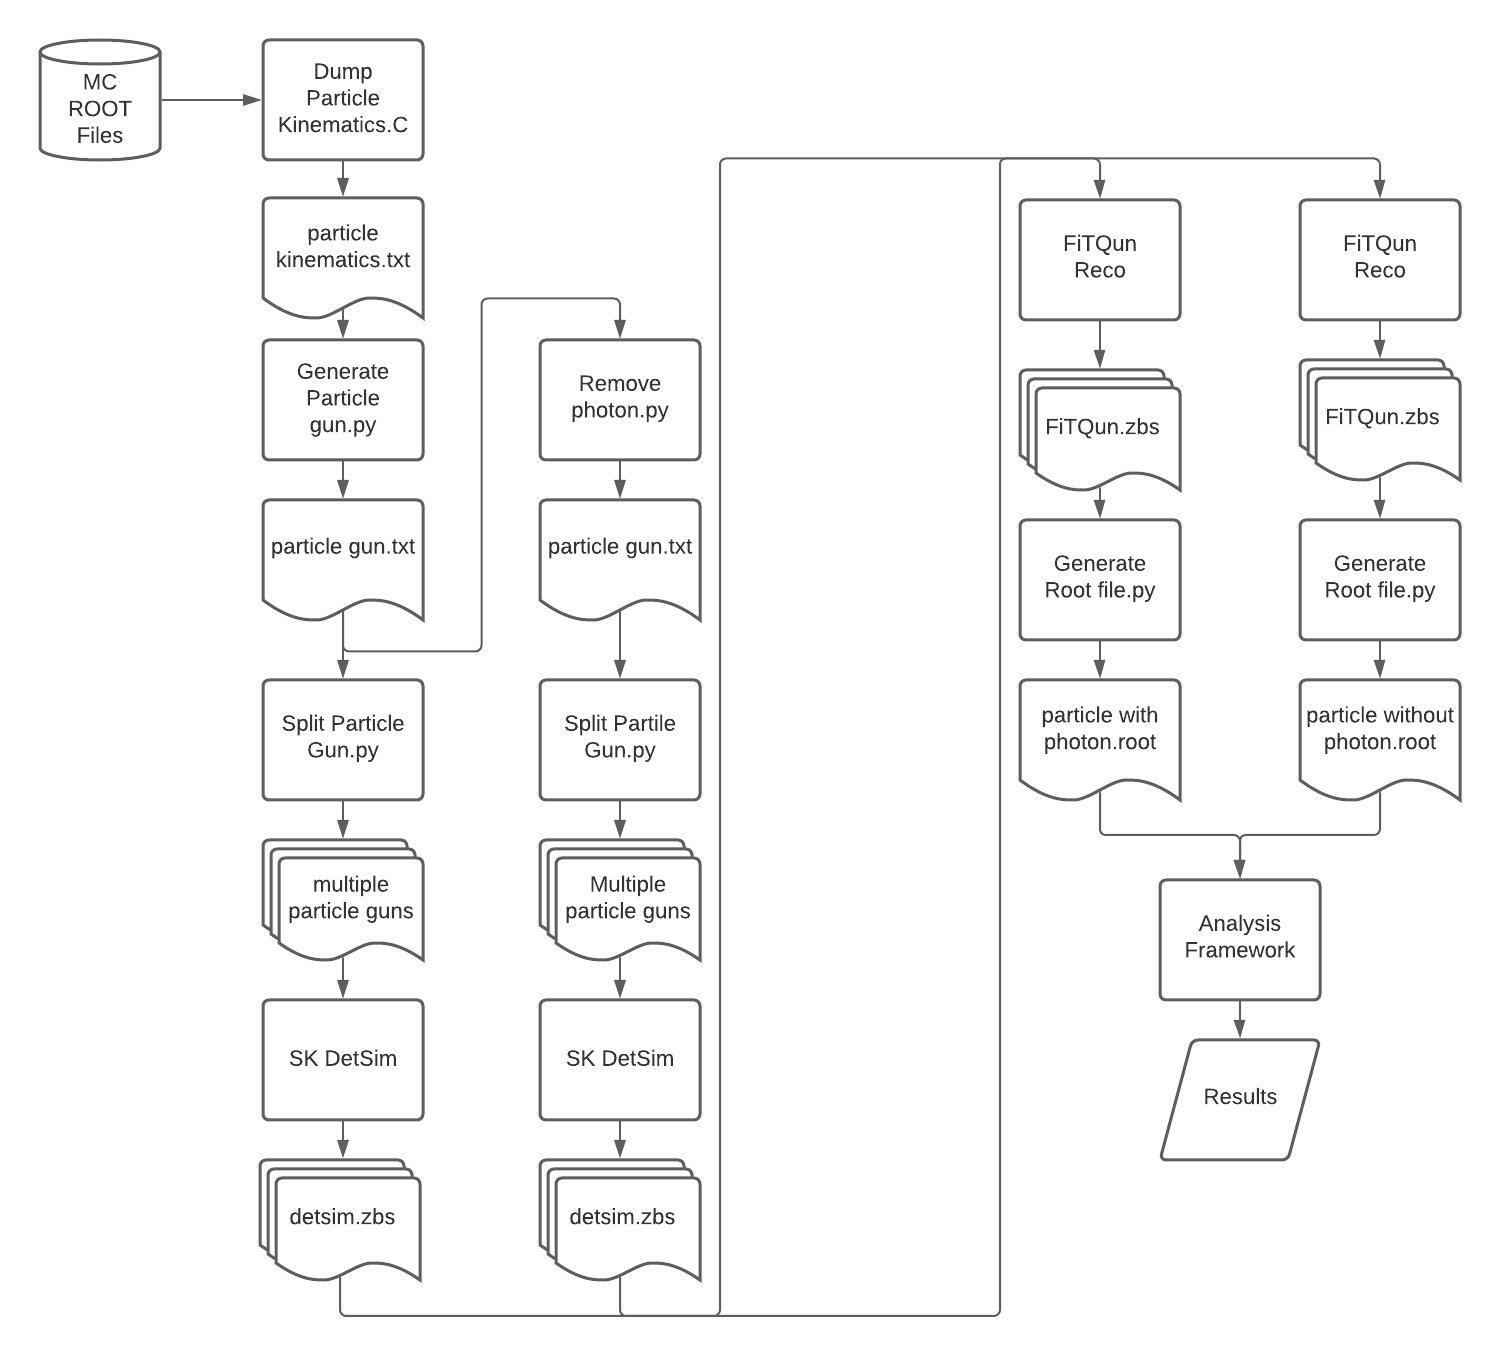
\includegraphics[scale=0.5]{radcorr_sw_framework.jpeg}
	\caption{Radiative Correction Framework}	
	}
\end{figure}
\begin{thebibliography}{9}
	\bibitem{Ko_phd} 
	Konosuke Iwamoto. 
	\textit{Neutrino Oscillation Measurements with An Expanded Electron Neutrino Appearance Sample in T2K, 2017.}
	
	%	\bibitem{Pueh_msc} 
	%	Pueh Leng Tan.
	%	\textit{Study of QED radiative corrections to
	%		charged lepton leg in neutrino-nucleon
	%		interactions, 2013.} 
	
	\bibitem{Kevin_talk1} 
	Kevin McFarland and Konosuke Iwamoto.
	\textit{Radiative CCQE and T2k's Oscillation Analyses, 2018}
	
	\bibitem{Rujula_calc}
	A. De Rujula, R. Petronzio and A. Savoy-Navarro
	\textit{Radiative Corrections to High-Energy Neutrino Scattering. Nucl.Phys. B154 (1979) 394. CERN-TH-2593.}
	
\end{thebibliography}
	
\end{document}

